\chapter{Generazione dei video fake}

\section{Funzionamento}

\section{Valutazione delle soluzioni disponibili}

Per la generazione dei video fake, sono stati valutati tre applicativi diversi, forniti come Software-as-a-Service (SaaS):
\begin{itemize}
    \item DupDub.com
    \item Synthesia.io
    \item HeyGen.com
\end{itemize}

I criteri che sono stati valutati sono: la naturalezza dei movimenti generati, l'estensione di questi ultimi, la qualità del lip-sync\footnote{sincronizzazione tra il movimento delle labbra di un soggetto e il suono delle parole pronunciate.}, la qualità e la naturalezza della voce parlata generata, e il grado di realismo generale dato dai video generati. Vediamo per ordine i punti di forza e di debolezza identificati di ognuno, e come si è pervenuti alla scelta finale. 

\subsection{DupDub}

DupDub si classifica come un prodotto "Talking-Photo". A partire da una fotografia di un persona, genera il movimento dei muscoli facciali e delle labbra per simulare il parlato. DupDub trova i suoi punti di forza nell'essere molto semplice, ma è stato valutato come troppo semplice per gli scopi di questa ricerca. La più grande limitazione è data dalla limitatezza dei movimenti, limitandosi appunto a generare solo movimenti dei muscoli facciali, e a malapena movimenti della testa, rendendo il risultato finale poco convincente e innaturale. Inoltre, tutti gli avatar forniti dalla piattaforma per la generazione dei video sono chiaramente soggetti non reali, bensì generati a loro volta tramite IA.

\subsection{Synthesia.io}

Rispetto al precedente, Synthesia.io si mostra molto più capace. Fornisce avatar in mezzo busto, ed è in grado di generare movimenti del viso, della testa, e anche del corpo, producendo risultati decisamente più naturali di DupDub. Gli avatar forniti sembrano essere stati generati a partire da persone reali, ed il servizio offre la possibilità di generare avatar personali. I punti di debolezza individuati sono stati: la qualità del lip-sync e la qualità delle voci generate. In particolare, risultava frequente il disallineamento tra il movimento delle labbra dell'avatar e il suono della voce generato. La voce inoltre è stata valutata come poco espressiva e poco naturale. Vedremo in realtà come questi sono spesso i punti più deboli di questa tecnologia.

Nonostante questo, tale servizio sembrava un buon candidato per la ricerca, ma è stato scartato in base al piano offerto, in quanto offriva un servizio ad abbonamento basato su minuti. % Vi era un numero limitato di minuti di video generabili al mese, il che avrebbe limitato/rallentato il processo di ricerca.

\subsection{HeyGen}

Sin dal primo sguardo, HeyGen.com si è dimostrato essere al di sopra di tutti gli altri, offrendo anche la possibilità di generare video su sfondi reali, angolazioni diverse dello stesso avatar, e implementando movimenti del corpo avanzati come il movimento delle braccia e il gesticolamento delle mani. Gli avatar sono costruiti a partire da un video di riferimento del soggetto, il che li conferisce la possibilità di apprendere ed emulare i movimenti della persona inquadrata, producendo un risultato più naturale e realistico. Inoltre, la piattaforma si è dimostrata essere in constante evoluzione e sviluppo, arricchendo il suo catalogo di funzionalità, avatar e di voci durante il periodo di valutazione.

Per queste ragioni, tra le opzioni valutate, HeyGen è stato decretato come il migliore, in termini di qualità e naturalezza dei risultati prodotti, ed è stato quindi scelto come soluzione per la nostra ricerca. Un altro fattore che sicuramente ha giocato a suo favore è stato anche il piano offerto, il quale ci ha permesso di generare infiniti video durante il periodo di abbonamento, posto che questi fossero sotto i cinque minuti di durata.

\paragraph{Profilo dei video fake}
Si delinea così il tipo di video che siamo in grado di generare: gli avatar sono privi di sfondo, per cui i video fake sono video con sfondo bianco, statici, privi di movimenti di macchina o cambi di inquadrature, e sono privi di animazioni o scritte che compaiono a corredo.

\section{Video real}

Identificata la piattaforma per la generazione dei video fake, è necessario procurarsi i video reali da utilizzare come riferimento per generare tali doppioni fake. Il tipo di video richiesto per i video real sono dei video brevi (durata inferiore ai 5 minuti), in modo che possano essere visti per intero. Fondamentale è trovare dei contenuti che non richiedano una particolare formazione pregressa per la loro comprensione, ma che non siano neanche banali, in modo di poter fare delle domande di comprensione a loro volta non banali. 

\subsection{Scelta dei video real}

\paragraph{Criterio di scelta}
È stata utilizzata per la ricerca dei video la piattaforma YouTube, e il criterio di ricerca dei video reali è semplice: cercare i video più simili possibili ai video fake che siamo in grado di generare. Per tali ragioni, il criterio di scelta consiste in:
\begin{itemize}
    \item video frontali, con un soggetto al centro e sfondo bianco
    \item nessun movimento di macchina o cambi di inquadrature
    \item autodescrittivo, in altre parole video dove non vengono utilizzate immagini, slide o grafici di supporto che vengono esplicitamente referenziati dallo speaker\footnote{questo perché contenuti esplicitamente referenziati dallo speaker reale non sarebbero presenti nel corrispettivo video fake, rompendo l'illusione.}
    \item video con il minor numero di scritte o immagini che compaiono a corredo, preferibilmente nessuna
    \item video con i sottotitoli preferibilmente inseriti a mano dall'autore del video, in modo da poter scaricare il copione associato al video più facilmente
\end{itemize}

\paragraph{Video trovati}

Per la realizzazione di un pilot della ricerca, sono stati identificati quattro video che soddisfano i criteri stabiliti:
\begin{itemize}
    \item \textit{"How to make a GREAT impression - Presentation Tips"} di Expert Academy %(https://youtu.be/lZg6H0WqPVY)
    \item \textit{"How to start a pitch or presentation"} di Dominic Colenso %(https://youtu.be/P2LwuF7zn9c)
    \item \textit{"How to start a presentation"} di Expert Academy %(https://youtu.be/LrjlW00kkws)
    \item \textit{"How to Get Over Your Fear of Public Speaking"} di Expert Academy %(https://youtu.be/So3Z93hEPDk)
\end{itemize}

I video sono stati scaricati utilizzando il tool open source \verb|yt-dlp| (\url{https://github.com/yt-dlp/yt-dlp}).

\subsection{Processing}

I video individuati non corrispondevano tutti perfettamente alle specifiche richieste, per cui per poterli integrare nella ricerca, è stato necessario fare del pre-processing.

\subsubsection{Trimming}

Tutti i video individuati presentavano un introduzione e una coda al video, con musiche, scritte ed elementi animati. I video individuati sono per cui stati tagliati, in modo da eliminare gli elementi non utili al nostro studio, e mantenere solamente la parte di video parlata. Per il trimming dei video è stato utilizzato il tool open source gratuito \verb|ffmpeg| (\url{https://www.ffmpeg.org}), così da favorire un'operazione veloce e priva di operazioni di re-econding ove possibile.

\subsubsection{Pulizia dello sfondo}

Alcuni dei video individuati inoltre presentavano alcuni elementi grafici a comparsa durante la parte parlata del video, come grafici o piccole scritte. Questo è stato valutato come accettabile visto che tali elementi non venivano referenziati esplicitamente dallo speaker, e comparivano solo in sovrapposizione dello sfondo.\footnote{Ricordiamo che tutti i video individuati presentano uno sfondo bianco uniforme, che non cambia nel tempo.} Questo ha permesso la rimozione di tali elementi aggiuntivi tramite una semplice operazione di video-editing, detta mascheramento.

\paragraph{Mascheramento}

Si identifica un fotogramma dell'immagine dove non vi sono elementi a coprire la parte dello sfondo interessata, e si salva tale fotogramma come file a parte. Questo fotogramma "pulito" è detto \textit{clean plate}. Dal momento che lo sfondo è statico, ovvero non cambia nel tempo, il clean plate funge da copia pulita dell'immagine, che possiamo utilizzare per coprire qualunque elemento che compare in sovrapposizione dello sfondo. Con un qualunque programma di editing, si sovrappone il clean plate alla porzione temporale di video in cui compare l'elemento da rimuovere, ad esempio una scritta. Si effettua poi una maschera, che va a ritagliare il clean plate, in modo che, come una toppa, vada a coprire il testo in sovra-impressione, rimuovendolo dal video.

\begin{figure}[ht]
    \centering
    \begin{subfigure}{0.32\textwidth}
        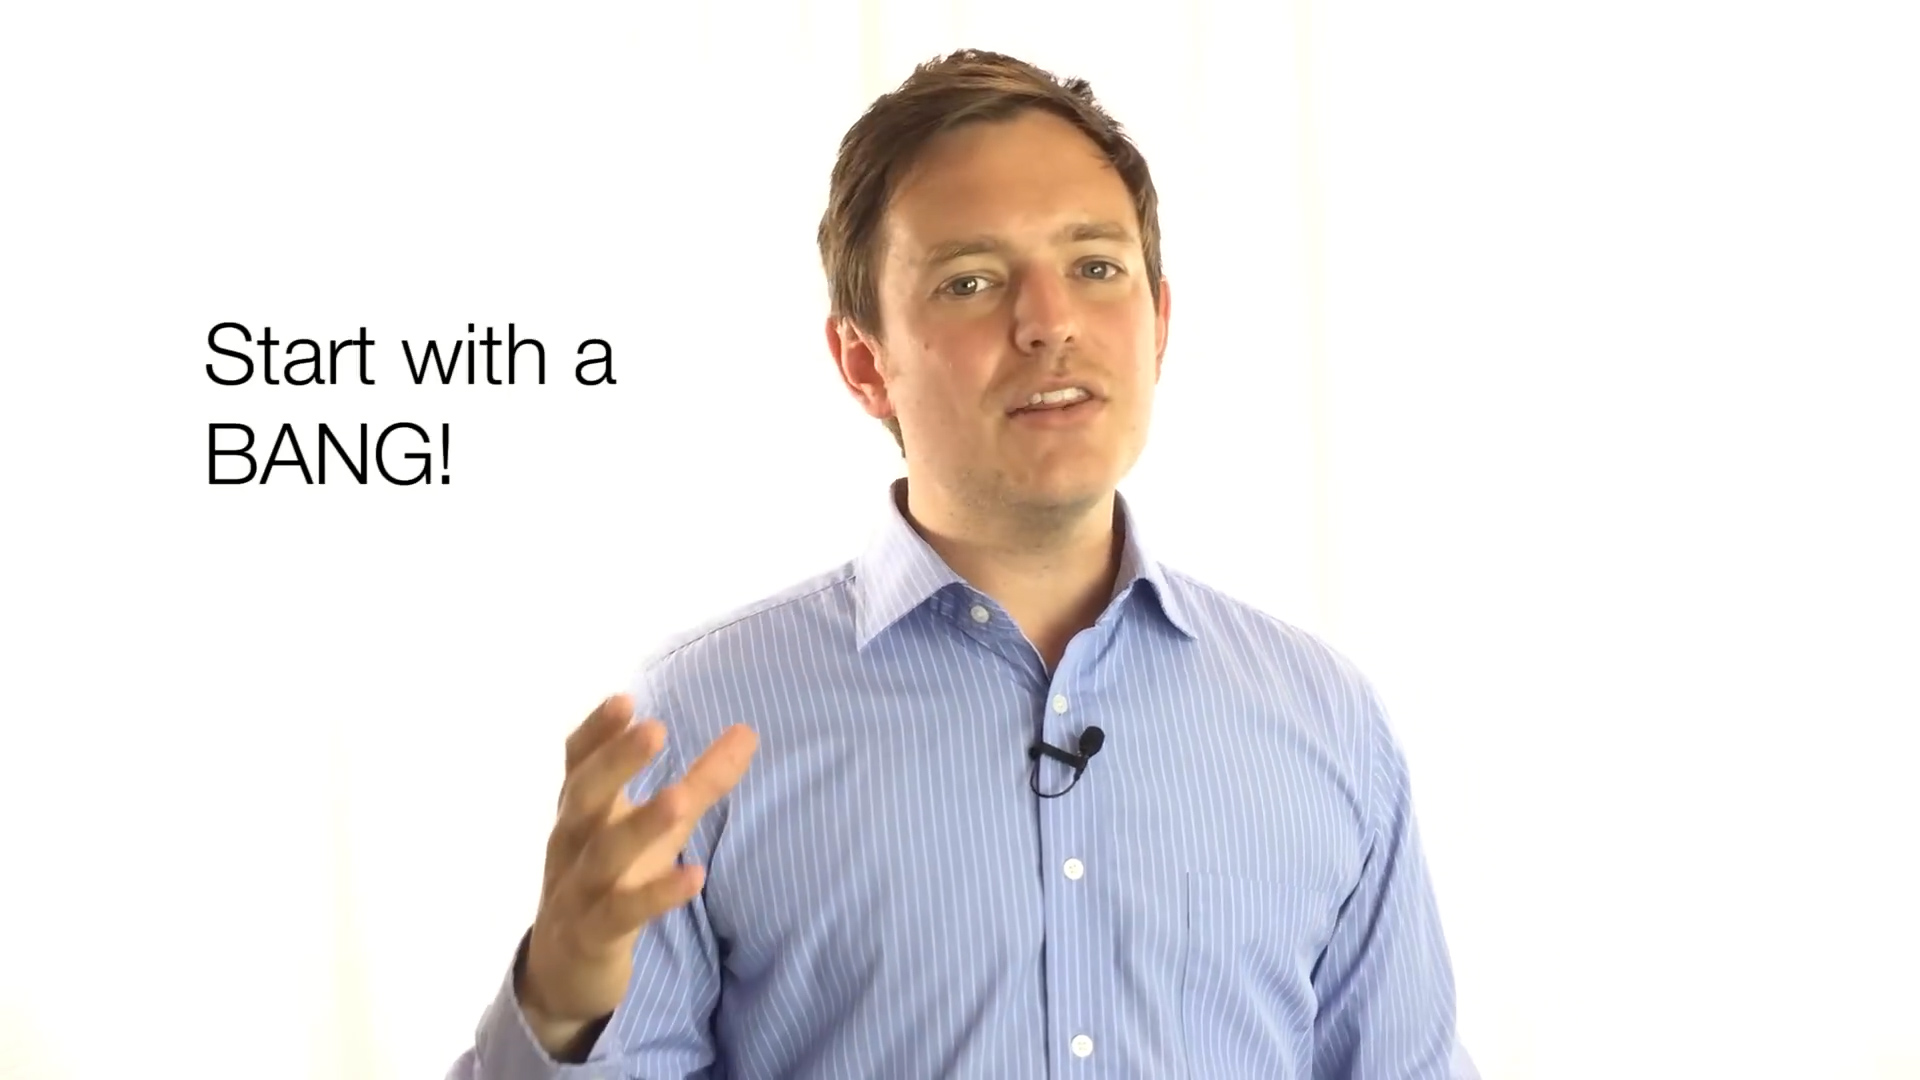
\includegraphics[width=0.95\linewidth]{images/original_frame} 
        \caption{Fotogramma originale}
        \label{fig:original_frame}
    \end{subfigure}
    \hfill
    \begin{subfigure}{0.32\textwidth}
        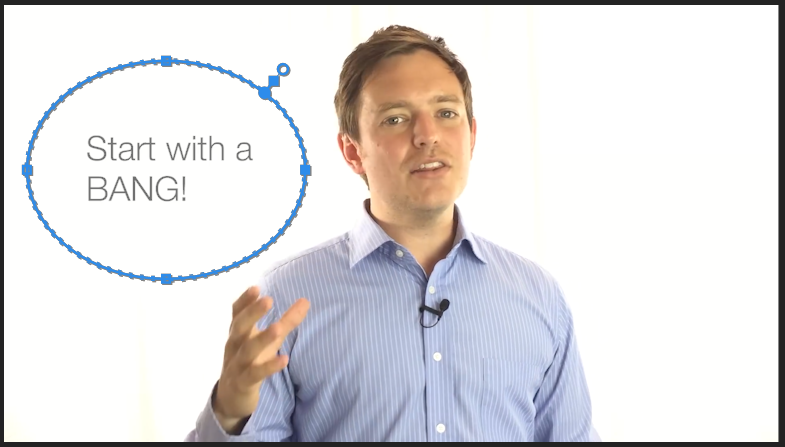
\includegraphics[width=0.95\linewidth]{images/mask_with_text}
        \caption{Maschera sovrapposta}
        \label{fig:mask_with_text}
    \end{subfigure}
    \hfill
    \begin{subfigure}{0.32\textwidth}
        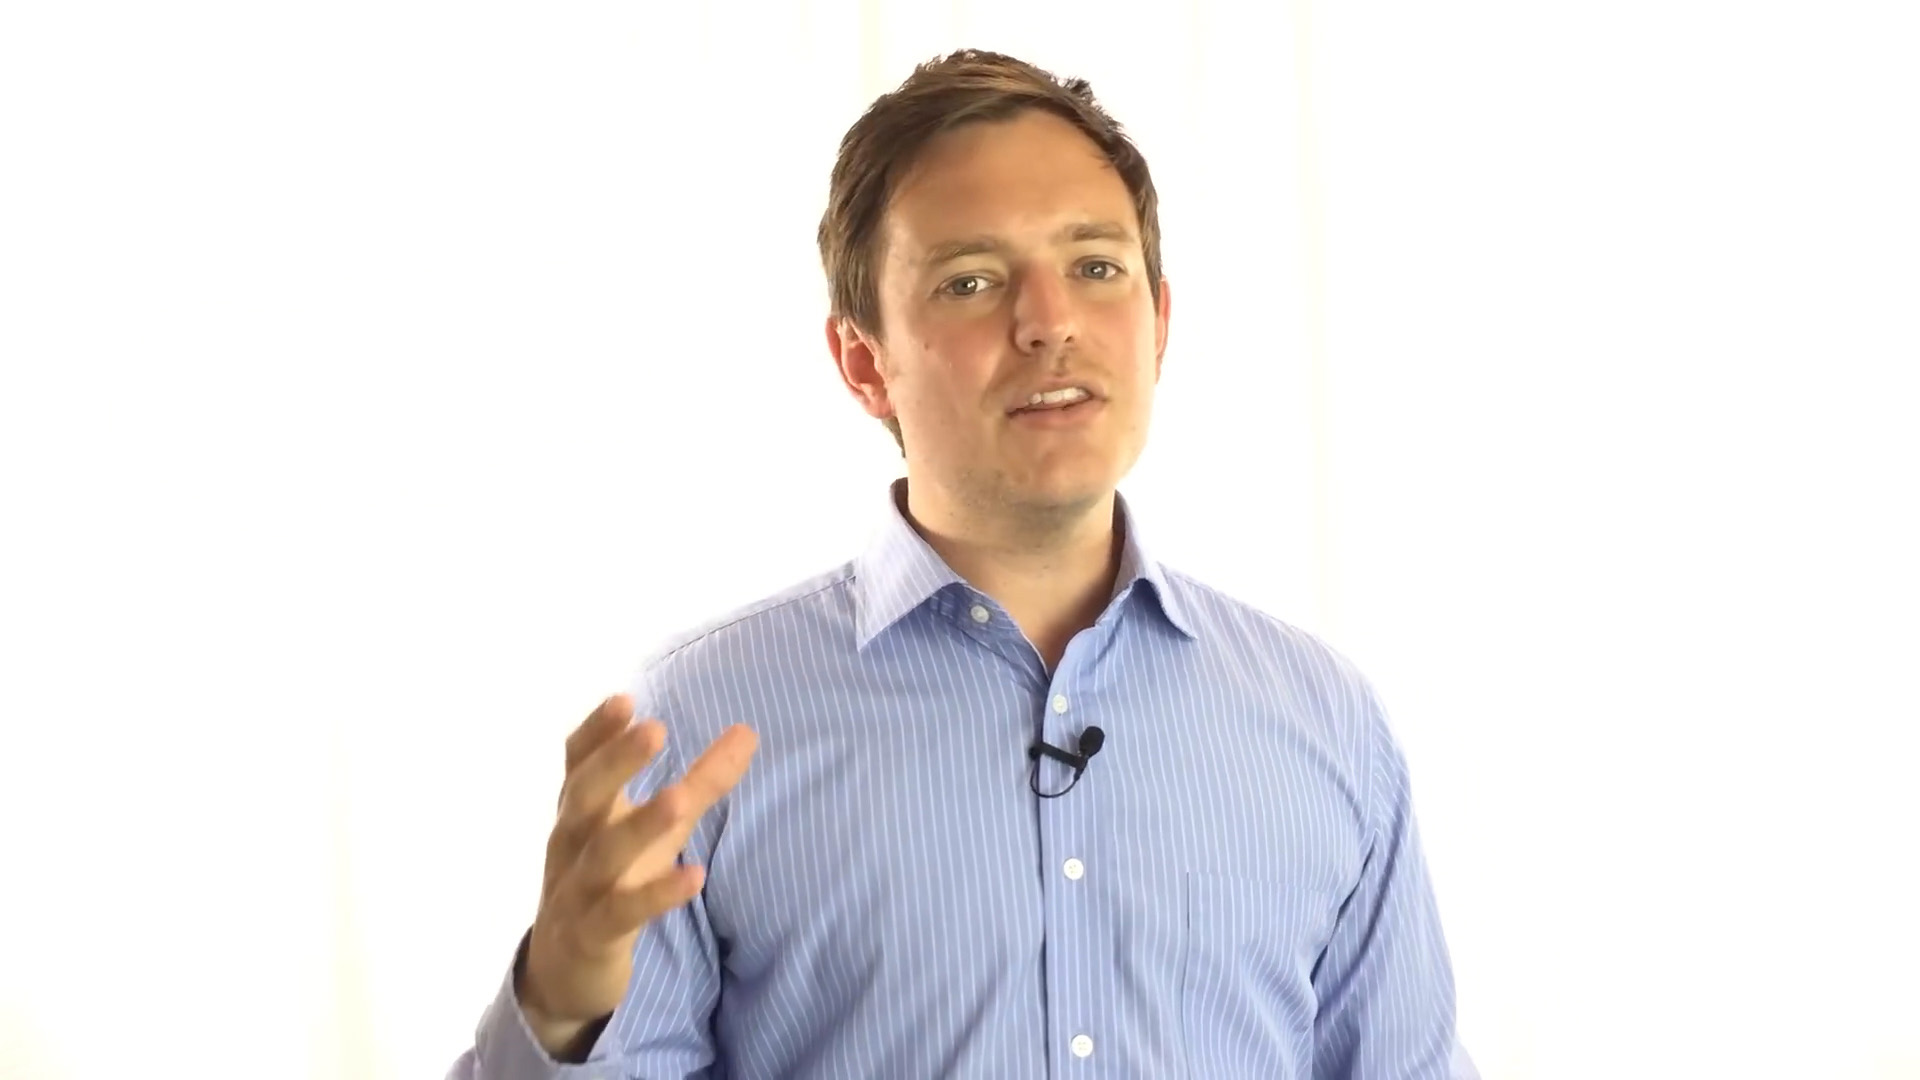
\includegraphics[width=0.95\linewidth]{images/masked}
        \caption{Fotogramma mascherato}
        \label{fig:masked}
    \end{subfigure}
    
    \caption{Una operazione di mascheramento con clean plate in Adobe Premiere Pro}
    \label{fig:masking}
\end{figure}

\subsubsection{Estrazione del testo}

Per poter generare i doppioni fake, è stato estratto il testo associato al parlato presente nei video individuati. È stato utilizzato il sito web gratuito \url{https://downsub.com} per scaricare i sottotitoli già forniti da YouTube. La maggior parte dei video presentavano dei sottotitoli ufficiali, ovvero inseriti direttamente dagli autori dei video. Per gli altri, sono stati scaricati i sottotitoli generati automaticamente da YouTube, utilizzando quindi di fatto il motore SpeechToText integrato di YouTube.

In ogni caso, tutti i sottotitoli scaricati sono stati poi revisionati a mano per eliminare refusi, errori di battitura o di trascrizione, e per eliminare elementi non parlati o associati alle parti di video che sono state tagliate via. Questi file di sottotitolo sono tutto il necessario per generare i video fake.

\section{Generazione dei video fake}

\clearpage